%%%%%%%%%%%%%%%%%%%%%%%%%%%%%%%%%%%%%%%%%%%%%%%%%%%%%%%%%%%%%%%%%%%%%
%
%  This is a sample LaTeX input file for your contribution to
%  the M&C2023 topical meeting.
%
%  Please use it as a template for your full paper
%    Accompanying/related file(s) include:
%       1. Document class/format file: mc2023.cls
%       2. Sample PDF/Postscript Figure: figure.pdf,figure.ps
%       3. A PDF file showing the desired appearance: mc2023_template.pdf
%       4. cites.sty and citesort.sty that might be needed by some users
%    Direct questions about these files to: buijsa@mcmaster.ca
%    Originals provided by brantley1@llnl.gov
%
%    Notes:
%      (1) You can use the "dvips" utility to convert .dvi
%          files to PostScript.  Then, use either Acrobat
%          Distiller or "ps2pdf" to convert to PDF format.
%      (2) Different versions of LaTeX have been observed to
%          shift the page down, causing improper margins.
%          If this occurs, adjust the "topmargin" value in the
%          mc2023.cls file to achieve the proper margins.
%
%%%%%%%%%%%%%%%%%%%%%%%%%%%%%%%%%%%%%%%%%%%%%%%%%%%%%%%%%%%%%%%%%%%%%


%%%%%%%%%%%%%%%%%%%%%%%%%%%%%%%%%%%%%%%%%%%%%%%%%%%%%%%%%%%%%%%%%%%%%
\documentclass[letterpaper]{mc2023}
%
%  various packages that you may wish to activate for usage
\usepackage{tabls}
\usepackage{cites}
\usepackage{epsf}
\usepackage{appendix}
\usepackage{ragged2e}
\usepackage[top=1in, bottom=1in, left=1in, right=1in]{geometry}
\usepackage{enumitem}
\setlist[itemize]{leftmargin=*}
\usepackage{caption}
\captionsetup{width=1.0\textwidth,font={bf,normalsize},skip=0.3cm,within=none,justification=centering}

% ELIMINATING WHITESPACE
\setlength{\belowcaptionskip}{-15pt}
\setlength{\abovedisplayskip}{4pt}
\setlength{\belowdisplayskip}{4pt}


\usepackage{xcolor}
\usepackage[colorlinks = true, linkcolor = black, urlcolor  = black, citecolor = black]{hyperref}
\usepackage{float} % for [H] option in figures

% GLOSSARIES
\usepackage[acronym,nomain,nonumberlist,nogroupskip,nopostdot]{glossaries} % for glossary of acronyms
\setacronymstyle{long-short}
\loadglsentries{glossary}
\makeglossaries
\renewcommand*{\glstextformat}[1]{\textcolor{black}{#1}} % make glossary color black

% Lewis custom commands
% This file contains custom commands that Lewis uses frequently in LaTeX documents

\usepackage{subcaption}
\usepackage{hyperref}
\hypersetup{colorlinks,allcolors=black}
% for more https://tex.stackexchange.com/questions/88400/hyperref-changing-the-linkcolor-locally-in-the-toc
\usepackage{amssymb}
\usepackage{bbm}

% matlab stuff
\usepackage{graphicx}
\usepackage{color}
\usepackage{matlab-prettifier}

%vector arrow
\usepackage{graphicx}
\newcommand{\cev}[1]{\reflectbox{\ensuremath{\vec{\reflectbox{\ensuremath{#1}}}}}}
% table packages
\usepackage{booktabs}
\usepackage{adjustbox}

% custom equation commands
\newcommand{\QOR}{\qquad \text{OR} \qquad}
\newcommand{\QAND}{\qquad \text{AND} \qquad}
\newcommand{\QTHUS}{\qquad \text{THUS} \qquad}
\newcommand{\QWITH}{\qquad \text{WITH} \qquad}
\newcommand{\QFOR}{\qquad \text{FOR} \qquad}
\newcommand{\QSO}{\qquad \text{SO} \qquad}
\newcommand{\QWHERE}{\qquad \text{WHERE} \qquad}
\newcommand{\QWHEN}{\qquad \text{WHEN} \qquad}
\newcommand{\LINE}{\par\noindent\rule{\textwidth}{0.4pt}\par}
\newcommand{\toinf}{\rightarrow\infty}
\newcommand{\tozero}{\rightarrow0}
\newcommand{\qeq}{\overset{?}{=}}
\newcommand{\ceq}{\overset{\checkmark}{=}}
\newcommand{\Poi}{\text{Poisson}}
\newcommand{\keff}{$k_{e\!f\!f}$}
\renewcommand{\epsilon}{\varepsilon} % squiggly epsilon

\def\brac#1{\{#1\}}
\def\Brac#1{\big\{#1\big\}}
\def\BRAC#1{\bigg\{#1\bigg\}}
\def\angbrac#1{\langle#1\rangle}
\def\Angbrac#1{\big\langle#1\big\rangle}
\def\ANGBRAC#1{\bigg\langle#1\bigg\rangle}
\usepackage{float}
% SI Units
\usepackage{siunitx}
\DeclareSIUnit\n{n}
\DeclareSIUnit\sp{sp}

\def\doubleunderline#1{\underline{\underline{#1}}}

\title{Verification of the Cardinal Multiphysics Solver for 1-D Coupled\\
Heat Transfer and Neutron Transport}

\raggedbottom % allows space at bottom of page, as opposed to verical justification
\author{%
  % FIRST AUTHORS
  %
  \textbf{L.I.~Gross$^1$, A.J.~Novak$^2$, P.~Shriwise$^2$, and P.P.H.~Wilson$^1$}\\
  $^1$University of Wisconsin -- Madison  \\
  1500 Engineering Drive, Madison, WI 53706 \vspace{6pt}\\
  $^2$Argonne National Laboratory \\
  9700 S Cass Avenue, Lemont, IL 60439\vspace{6pt} \\
  \url{ligross@wisc.edu}, \url{anovak@anl.gov}, \url{pshriwise@anl.gov} \url{paul.wilson@wisc.edu}
}
%
% Insert authors' names and short version of title in lines below
%
\newcommand{\authorHead}{Gross et al.}
\newcommand{\shortTitle}{Cardinal Multiphysics Analytical Benchmark Verification}
%
%%%%%%%%%%%%%%%%%%%%%%%%%%%%%%%%%%%%%%%%%%%%%%%%%%%%%%%%%%%%%%%%%%%%%
%
%   BEGIN DOCUMENT
%
%%%%%%%%%%%%%%%%%%%%%%%%%%%%%%%%%%%%%%%%%%%%%%%%%%%%%%%%%%%%%%%%%%%%%
\begin{document}
\maketitle
\justify
\parskip 6pt plus 1 pt minus 1 pt

\begin{abstract}
  Cardinal is a multiphysics software tool that couples OpenMC Monte Carlo transport and NekRS \gls{cfd} to the \gls{moose}.
  In this work, we verify Cardinal for coupled heat conduction and neutron transport using a 1-D analytic solution from previous
  work by the Naval Nuclear Laboratories. This numerical benchmark includes $S_2$ transport, Doppler-broadened cross-sections,
  thermal conduction and expansion, and convective boundary conditions. The goals of this work are to verify Cardinal's basic
  multiphysics modeling capabilities for coupled neutronics and heat conduction. The benchmark provides analytical solutions for
  the temperature and flux distributions, as well as the $k$-eigenvalue. Using these solutions, an $L_{2}$ error norm was computed
  for each spatial discretization (finite element heat conduction mesh, Monte Carlo cells). The temperature error showed linear
  convergence on a log-log plot of mesh element number vs error with a slope of $-0.9982$. \textit{The flux was near linear convergence,
  with a slope of  $-0.9496$ on a log-log plot of number of cells vs error, but the higher-than-expected error of the last
  element deviated from linear behavior.}
  % The ratio of the \gls{ce} temperature and flux in each mesh element shows agreement as the \gls{ce} for each mesh approaches
  % the ideal $y=1$ as the mesh size increases. Both plots show that with increasing mesh elements, the \gls{ce} approaches the
  % ideal $y=1$.
  The eigenvalue $k_{eff}$ agrees well with the benchmark value for each mesh size. The outcome of this work is verification of coupled
  Monte Carlo-thermal conduction modeling using Cardinal.
\end{abstract}
\vspace{6pt}
\keywords{Cardinal, MOOSE, OpenMC, multiphysics, verification}

\section{INTRODUCTION}
\label{sec:intro}
With recent advancements in methods, software, and computing, high-fidelity multiphysics \gls{ms} is becoming an important
component of the nuclear engineer's ``toolbox.'' These high-fidelity models substitute more conservative safety factors
with predictive science. This can reduce uncertainty in analyses, enabling tighter margins to realize improved economics
and licensing certainty. However, analytical benchmarks and comparison to experimental data are required to assess the stability,
convergence, and predictive capability of these high-fidelity models for reactor design and analysis.

Cardinal \cite{novak2022-cardinal,cardinal-website} (\url{https://cardinal.cels.anl.gov/}) is an open-source code that couples OpenMC
\cite{openmc} Monte Carlo particle transport and NekRS \gls{cfd} to \gls{moose} \cite{lindsay2022moose}. This coupling brings high-fidelity
multiphysics feedback to the \gls{moose} ``ecosystem.'' Cardinal couples OpenMC and NekRS to \gls{moose} simulations by copying data
between the internal code data structures (e.g. a vector of tally results in OpenMC) and a \texttt{MooseMesh}, or the unstructured mesh
class in \gls{moose}. \gls{moose}'s mesh-to-mesh interpolation system then communicates between the \texttt{MooseMesh} ``mirror'' of the
external code's solution and an arbitrary coupled \gls{moose} application in the form of boundary conditions (such as for conjugate heat
transfer with NekRS) or source terms (such as for volumetric heating with OpenMC). Convergence is obtained with Picard iteration.

For coupled neutronics-thermal-fluid simulations with OpenMC, each Picard iteration consists of several steps: 1)~a \gls{moose}
application (e.g. BISON, Pronghorn, NekRS via Cardinal, ...) solves for temperatures and densities; 2)~Cardinal transfers
temperatures and densities to the OpenMC model; 3)~OpenMC solves for the nuclear heating; and 4)~Cardinal transfers the tally
values to the \texttt{MooseMesh} ``mirror.''

These steps continue until convergence criteria is achieved. In this work, we pursue verification of these multiphysics aspects
of Cardinal using a 1-D analytical benchmark from the Naval Nuclear Laboratories \cite{analytical-benchmark}.  This work does
not require \gls{cfd}, and thus NekRS will be left out of the discussion from this point on.

The remainder of this paper is organized as follows. In Section \ref{sec:benchmark}, we summarize the analytical benchmark
modeled in this work. Section \ref{sec:model} then describes the Cardinal computational model of the benchmark. Section
\ref{sec:results} presents comparisons between Cardinal and the analytical benchmark. Finally, Section \ref{sec:conclusions}
presents conclusions and outlines ongoing and future efforts in the verification and validation of Cardinal.

\section{BENCHMARK PROBLEM DESCRIPTION}
\label{sec:benchmark}
The analytical benchmark couples three physics: $S_2$ neutron transport with Doppler broadening, heat conduction,
and thermal expansion. $S_{2}$ transport restricts the neutron direction to only the $\pm x$ direction. A summary of the governing
\glspl{ode} and boundary conditions in the 1-D slab is shown in Fig. \ref{fig:slab_diagram}.
\begin{figure}[H]
    \centering
    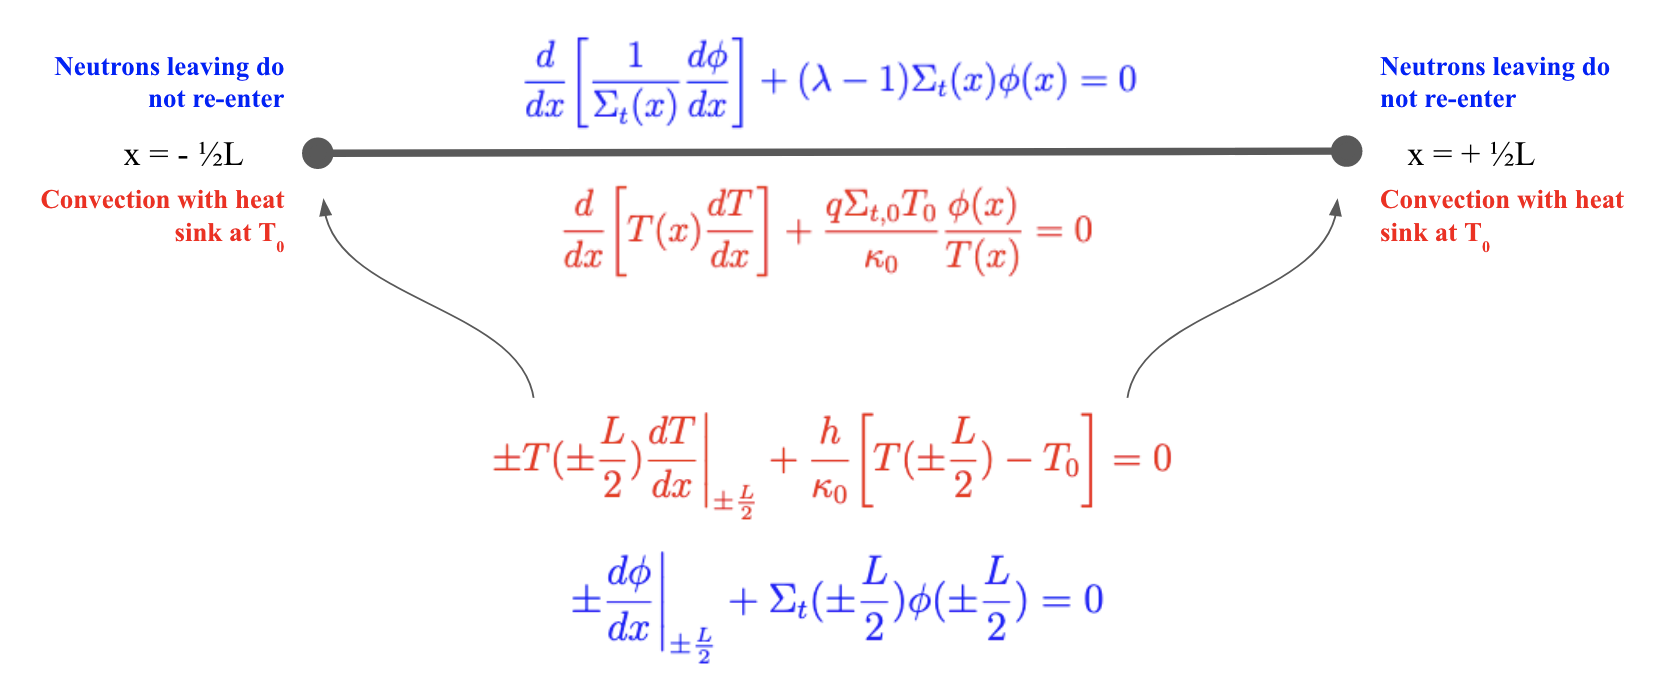
\includegraphics[width=0.85\linewidth]{figures/1D_Benchmark_Diagram.png}
    \caption{The domain, \glspl{ode}, and boundary conditions for the slab.}
    \label{fig:slab_diagram}
\end{figure}

This benchmark uses a one-group assumption for the neutron cross-sections. As neutrons transport, heat from fission events deposit
volumetric power in the slab, causing thermal expansion and affecting the temperature distribution; thermal expansion is restricted
to only the $x$-direction. This slab elongation feeds back into neutronics and heat conduction by influencing the domain length and
material density. The slab has convective boundary conditions at the endpoints $x=\pm \frac{L}{2}$ with the heat sink temperature
$T_{0}$. The Doppler-broadened total, microscopic cross-section follows an inverse-root temperature relationship,
\begin{equation}
    \sigma_{t}(x) = \sigma_{t,0}\sqrt{\frac{T_{0}}{T(x)}}.
\end{equation}
Due to thermal expansion, the slab density varies as
\begin{equation} \label{sec:intro:density}
    \rho(x) =  \rho_{0} \sqrt{\frac{T_{0}}{T(x)}}.
\end{equation}
This gives a Doppler-broadened, macroscopic, total cross-section that accounts for changes in density due to temperature as
\begin{equation} \label{sec:intro:doppler}
    \Sigma_{t}(x) = \frac{\rho_{0}\sigma_{t,0} N_{A}}{A} \frac{T_{0}}{T(x)} = \Sigma_{t,0}\frac{T_{0}}{T(x)} ,
\end{equation}
where $ \sigma_{t,0}$ is the total, microscopic cross-section at $T_{0}$, $N_{A}$ is Avogadro's number, and $A$ is the mass number
of the medium. The conduction equation governs heat flow in the slab and can be described in terms of the thermal conductivity
$\kappa\big(T(x)\big)$, the energy released per reaction $q$, the total, macroscopic cross-section $\Sigma_{t}$, and the neutron flux $\phi$.
\begin{equation}
     \frac{d}{dx}\bigg[\kappa\big(T(x)\big)\frac{dT(x)}{dx}\bigg] + q \Sigma_{t}(x)\phi(x) = 0.
\end{equation}
Note that typically $q$ represents the energy per fission, but in this benchmark, it is per total reaction. The main assumption
used to craft the analytical solution is that $T(x)=f\phi(x)$. This assumption is guaranteed by manipulating the \glspl{ode},
inserting the cross-section temperature dependence, and matching coefficients so that the two \glspl{ode} are of the same form.
The matching of coefficients imposes two constraints that give equations for the total, microscopic cross-section $\sigma_{t,0}$
and the heat transfer coefficient $h$, in terms of the slab parameters. For full details on the analytical solution's derivation,
see \cite{analytical-benchmark}.

\section{COMPUTATIONAL MODEL}
\label{sec:model}
This section describes the OpenMC and \gls{moose} computational models, followed by the convergence criteria used for coupling.
At the time at which this benchmark modeling was performed, Cardinal did not support moving geometries in OpenMC. Instead of
using thermomechanics for thermal expansion, our simulation simply uses the analytic solution for the equilibrium length $L$
from \cite{analytical-benchmark} that accounts for all three physics effects. The change in density due to temperature is
accounted for in this simulation by using the total, macroscopic cross-section\ --\ which absorbs density to become a
$\frac{1}{T}$ dependence\ --\ from (\ref{sec:intro:doppler}), as was mentioned in Section \ref{sec:benchmark}. We note that,
in a companion paper in this conference \cite{novak-2023}, that Cardinal now supports mesh-based geometry (and deforming-mesh
problems) through the DAGMC plugin, and hence incorporating the thermomechanics feedback will be included in our future work.


\subsection{OpenMC Model}
\label{sec:model:OpenMC}
The geometry used in OpenMC must be finite, despite the benchmark being infinite in the $y$ and $z$ directions. The slab
is divided evenly into $N$ identically shaped rectangular cells along the $x$-dimension; the cases here are $N=[50,100,250,500,1000]$
cells. In general, reflective boundary conditions can be used to simulate infinite dimensions. Thus, this benchmark can be
represented with vacuum boundary conditions at $x=\pm \frac{L}{2}$ and reflective boundary conditions at the $y$ and $z$ boundaries.
The cell boundaries have transmissive boundary conditions, which just allows particles to pass without modifying their state.
Note that particles only move in the $\pm x$ direction, so no $y$ or $z$ boundaries are crossed, but with non-$S_{2}$ scattering,
the reflective boundaries would come into play. In addition to being finite for the model, the $y$ and $z$ dimensions need to be
set to $1$ cm in order for Equation (19) from the benchmark to uphold its one dimensional power integral, i.e. that integration in
$y$ and $z$ is implied to contribute a factor of 1 \cite{analytical-benchmark}. Fig. \ref{fig:slab_diagram} shows a diagram
of the 1-D geometry, governing equations, and boundary conditions for the different physics.

The benchmark's one-group assumption was satisfied using OpenMC's multigroup mode. Since the benchmark uses a fictitious material
with a known function for the temperature dependence, the simulation took advantage of OpenMC's capability for user-defined
cross-sections via the \texttt{XSdata} class. The cross-section for each reaction was specified for 50 evenly spaced temperatures
between 308 K and 358 K (a range slightly larger than, but including the  analytic temperature range from the benchmark) and was
exported to a library. Then, when running OpenMC in multigroup mode, that library is loaded to determine the appropriate cross-section
in each region as temperature changed via input from Cardinal from iteration to iteration.

OpenMC required slight source code modifications to accommodate $S_2$-like transport. In typical OpenMC simulations,
the physics of each reaction describes the scattering dynamics. The Monte Carlo algorithm is agnostic to the direction
particles move, but it is not typically constrained to a discrete directional distribution. However, when modeling this
benchmark, any history with a particle moving perpendicular to the $x$-direction would attenuate particles in less
$x$-distance than if particles were constrained to either $\pm x$. To address this, we first use OpenMC's \texttt{PolarAzimuthal}
distribution to restrict the birth direction of particles to the $\pm x$ direction. We then also modified OpenMC in a
patched branch to mimic $S_{2}$ transport in two ways. First, when determining the angular cosine of scattering events,
$\mu$, particles either continue forward ($\mu=1$) or are back-scattered ($\mu=-1$) with equal probability, as opposed to
sampling the reaction physics for $\mu$. Second, since the simulation uses $k$-eigenvalue mode, neutrons born in subsequent
generations of the simulation also need to have their angular birth distributions restricted to $\pm x$.

Due to the stochastic nature of Monte Carlo, an adequate number of histories must be used to obtain estimators that have reasonable
uncertainties. In eigenvalue mode, there are inactive batches followed by active batches. The difference is that inactive batches run
the simulation, but do not tally the requested estimators. The only quantity that is tracked is the fission source, which is passed from
each inactive batch to the next. The goal is to converge the fission source before tallying, as the initial guess may be inaccurate.
Thus, the number of inactive batches is an important parameter. Shannon Entropy computations can help determine fission source convergence
\cite{brown-entropy-2006}. A Shannon Entropy study for this system was conducted on the 1000 cell case, as increasing the cell size
improves statistics -- at least until there are too few cells to capture spatial dependence. This problem's analytical fission source
actually turns out to be independent of position, due to the multiplication of cross-section by flux, where the inverse $T$ and $T$
relationships cancel, so it is safe to assume that if the fission source converges for 1000 cells, it would converge for all the fewer
cell cases using the same number of histories. It was found the Shannon Entropy converges in fewer than 5 iterations. This may seem
like a low number, but the problem is 1-D and the initial guess provided to OpenMC is a uniform distribution, which is the same as the
actual converged solution. In order to be safe, the $k$-eigenvalue simulation used 50,000 particles per batch, with 50 inactive batches
and 50 active batches for every case.

A few tallies were used in order to compare to the analytical solution: a flux cell tally, a kappa-fission rate cell and global tally,
and the eigenvalue $k_{eff}$. Each tally uses a track-length estimator. As particles transport, their path may stay inside a given cell
or span more cells. The track-length estimator contributes a tally score when individual particle tracks passs through a region. Though
flux and the eigenvalue are the only quantities to compare with the benchmark, these other tallies are needed in order to compute a
source strength. OpenMC reports flux, denoted as $\hat{\phi}$, in units of $\frac{n-cm}{sp}$, where $sp$ indicates ``source particle.''
Typical flux, denoted as $\phi$, has units of $\frac{n}{cm^2-s}$. In fixed source modes, the source strength is typically known, but in
eigenvalue mode, it must be computed, as it depends on the physical source and fission source. The source strength is given by
\begin{equation} \label{eq:source_strength}
   \text{source strength} = \frac{P}{kf V_{cell}} \QTHUS \phi = \frac{P}{kf V_{cell} }\hat{\phi},
\end{equation}
where $P=1e22 \frac{ev}{s}$ is the slab integrated power from the benchmark, $kf$ is the tallied kappa-fission rate across the slab,
and $V_{cell}$ is the volume the cell containing the tally. The same source strength could be used to convert the kappa-fission tally from
OpenMC, which has units of $\frac{ev}{sp}$, to more physically meaningful units of $\frac{ev}{cm^3-s}$.

\subsection{MOOSE Heat Conduction Model}
\gls{moose} is used to solve for the temperature distribution within the slab via the Heat Conduction Module. In this \gls{moose}
model, a mesh is used that has identical dimensions to the cells used in the OpenMC model. While this is not required by Cardinal,
it allows for 1-to-1 feedback between the temperature computed in \gls{moose} and the heat source computed in OpenMC. \gls{moose}
solves the conduction equation using the \gls{fem}:
\begin{equation}\label{eq:conduction}
    - \nabla \cdot (\kappa_{s}(\mathbf{r},T_{s}) \nabla T_{s}(\mathbf{r})) = \dot{q}_{s},
\end{equation}
where $\kappa_{s}$ is the thermal conductivity in the solid and $\dot{q}_{s}$ is the heat source, in this case from fission. The
boundary conditions used by \gls{moose} match temperature boundary condition in red shown in Fig (\ref{fig:slab_diagram}). \gls{moose}
is coupled to OpenMC by receiving the heat source in each element from the kappa-fission tally. During each constituent iteration,
it recomputes the temperature distribution from the heat source and boundary conditions, and then sends the temperatures back to
OpenMC for the next transport solve.

\subsection{Convergence Criteria}
\gls{moose} uses iterative methods to compute temperature. It uses a combination of linear and non-linear iterations to update the
solution. It begins with a non-linear iteration, then linear iterations are run until convergence criteria are met. These trigger the
next non-linear iteration and this process repeats until both of the convergence criteria are met. This study used convergence criteria
of $10^{-7}$ for absolute tolerance and $10^{-9}$ for relative tolerance. Monte Carlo is a stochastic method, so convergence is achieved
by using an appropriate number of batches and histories per batch. The configurations used here were mentioned in Section
\ref{sec:model:OpenMC}.

In terms of converging global iterations across all single physics, each mesh cases used 200 Picard Iterations. To assist with
convergence of Monte Carlo quantities, Robbins-Monro relaxation was applied to the flux and kappa-fission tallies. This updates the
quantities of interest for the $n+1$th iteration as an average over the newest solution and the $n$ previous iterations \cite{dufek}.
So the flux at Picard Iteration $n$ would be given by
\begin{equation}\label{eq:Robbins-Monro}
    \Phi_{n} = \frac{1}{n+1} \sum_{i=0}^{n} \phi_{i},
\end{equation}
where $\Phi_{n}$ is the relaxed flux at step $n$ and $\phi_{i}$ is the flux output from the $i$th Monte Carlo solve. In order to
assess the convergence of each physics, plots of error versus mesh element size were used and will be shown in Section \ref{sec:results}.

One \gls{moose} convergence feature that was not used here is steady-state detection. By setting a steady-state tolerance, \gls{moose}
will iterate until the solution norm changes by less than this tolerance. In this benchmark, a high number of Picard Iterations was used
in order to ensure convergence, but other modelers may not want to incur the computational cost of running 200 Picard Iterations. They can
use steady-state detection instead.

\section{RESULTS}\label{sec:results}
The results to compare with the benchmark are the temperature distribution, flux distribution, and $k$-eigenvalue. The benchmark provides
analytical solutions for all of these quantities. An example temperature distribution is shown in the figure below for the 50 mesh element case.
\begin{figure}[H]
    \centering
    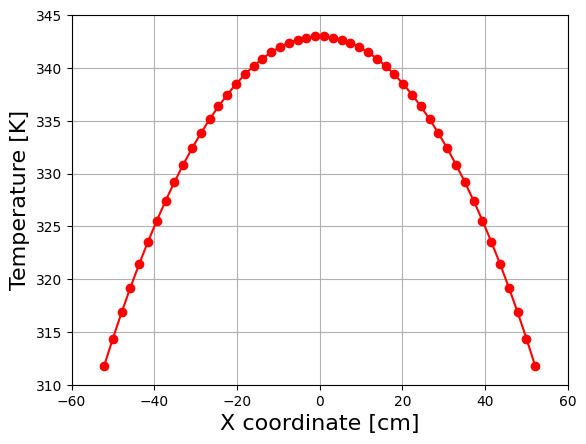
\includegraphics[width=0.55\linewidth]{figures/temp_50.png}
    \caption{The computed temperature for 50 mesh elements.}
    \label{fig:temp50}
\end{figure}
In order to assess the accuracy of the temperature solution and verify that refining the mesh increases the accuracy, the analytical solution
was used to compute an $L_{2}$ error norm for temperature. The error computed, $\epsilon_{T}$, is given by
\begin{equation}
    \epsilon_{T} = \frac{|| T_{a} - T_{x} ||_{2}}{|| T_{a} ||_{2}},
\end{equation}
where $T_{a}$ is the analytical solution evaluated at the $x$-centroid of each mesh element and $T_{x}$ is the temperature computed for that
voxel from the multiphysics simulation. The figure below shows how the temperature error norm relates to the number of mesh elements
\begin{figure}[H]
    \centering
    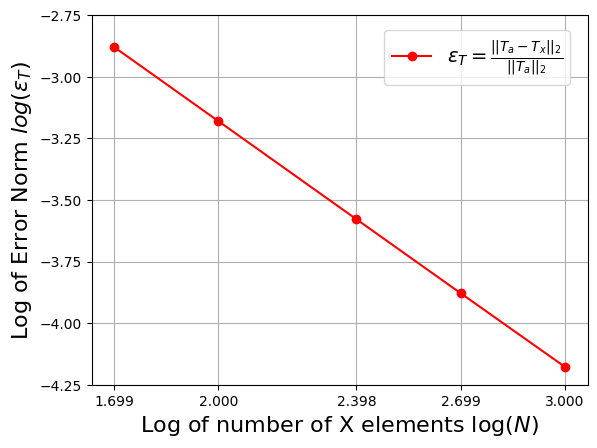
\includegraphics[width=0.65\linewidth]{figures/temp_error_norms.png}
    \caption{The number of mesh elements vs the log of the $L_{2}$ error norm for the computed vs analytical temperature.}
    \label{fig:temp_error_study}
\end{figure}
Linear convergence is achieved, as the slope of the line on the $\log(N)$ vs $\log(\epsilon_{T})$ plot is $-0.9981$. The same convergence test
was used on the flux solution as well. The flux error norm, $\epsilon_{\phi}$, is defined as
\begin{equation}
    \epsilon_{\phi} =  \frac{|| \phi_{a} - \phi_{x} ||_{2}}{|| \phi_{a} ||_{2}}.
\end{equation}
The figure below shows how the flux error norm relates to the number of mesh elements
\begin{figure}[H]
    \centering
    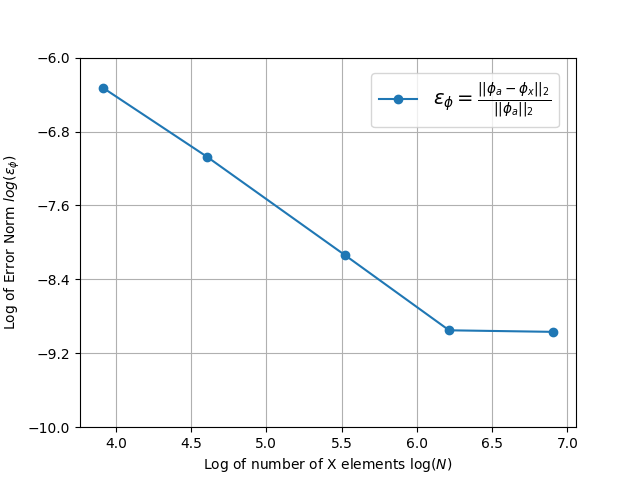
\includegraphics[width=0.65\linewidth]{figures/flux_error_norms.png}
    \caption{The number of mesh elements vs the log of the $L_{2}$ error norm for the computed vs analytical flux.}
    \label{fig:flux_error_study}
\end{figure}
The slope of the line of best fit for $\log(N)$ vs $\log(\epsilon_{\phi})$ plot is $-0.9496$. This deviation from first order is clearly being
caused by the error in the finest case ($N=1000$). The error for the $N=1000$ cases does decrease compared to $N=500$, but not be enough to fall in
line with linear convergence. This is the case where the volume of each cell/element is the smallest. In Monte Carlo, as the volume of a region holding
a tally gets smaller, fewer events will happen in that region per history, and thus more histories are required to get the same uncertainty. The
$N=1000$ case appears to be experiencing issues related to the element size. One possible source of error could be the refinement in the cross-section
temperature library. All cases used a library with $50$ temperatures, so it is possible that this case is reaching a limit where more data refinement
would be required to achieve the expected convergence that matches the other cases.

While this case appears to not perform as well from the $L_{2}$ error norm, it performs will in another measure of comparison -- the \gls{ce}. The
\gls{ce} is the ratio between the computed quantity, $C$, and the expected answer, $E$. In this case, $C$ would either be the temperature or flux
output from Cardinal, and $E$ would be the corresponding analytical solution. Thus, the \gls{ce} ratio $r$ is given by
\begin{equation} \label{eq:ce}
   r  = \frac{C}{E}.
\end{equation}
The ideal would be exact equality, or a ratio of $r=1$. The temperature and flux \glspl{ce} for each mesh element and cell, respectively, are shown in the
figure below.
\begin{figure}[H]
    \centering
    \begin{minipage}[b]{0.495\linewidth}
        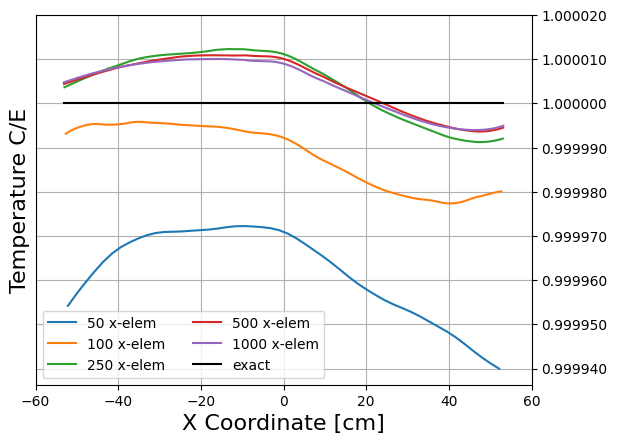
\includegraphics[width=\linewidth]{figures/temp_num_to_analy_ratios.png}
    \end{minipage}
    \begin{minipage}[b]{0.495\linewidth}
        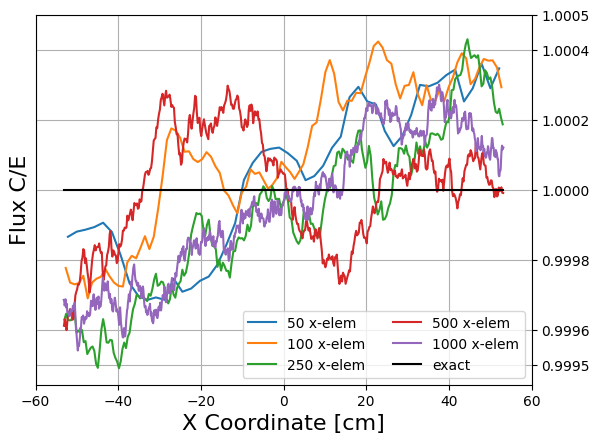
\includegraphics[width=\linewidth]{figures/flux_num_to_analy_ratios.png}
    \end{minipage}
    \caption{The left shows the \gls{ce} for temperature on every mesh and the right shows the \gls{ce} for flux in each cell.}
\end{figure}
Despite the disagreement from linear convergence for the flux, the \gls{ce} for the $N=1000$ case appears to be the closest to the line $y=1$. This
builds confidence that Cardinal is outputting a correct flux distribution for this case. The eigenvalue for each mesh is reported in the table below.
\begin{table}[H]
    \centering
    \caption{Eigenvalue with uncertainty for each mesh size, and the pcm difference from the analytical.}
    \begin{tabular}{@{}ccc@{}}
        \toprule
        \multicolumn{3}{c}{analytical $k_{eff}=0.29557$} \\
        \midrule
        number of OpenMC cells & numerical $k_{eff}$ & pcm (analytical - numerical)\\
        \midrule
        50 & 0.29555 $\pm$ 0.00009 & -2 \\
        100 & 0.29551 $\pm$ 0.00011 & -6 \\
        250 & 0.29560  $\pm$ 0.00012 &  -3 \\
        500 & 0.29575 $\pm$ 0.00013 & 18 \\
        1000 & 0.29551 $\pm$ 0.00013 & -6 \\
        \bottomrule
    \end{tabular}
    \label{tab:data}
\end{table}
The eigenvalue is the metric that agrees with the analytical solution the quickest. This is due to it being a system-wide parameter, which gains
contributions from every fission event, no matter which cell they occur in. It converges much quicker than the flux, which only gains contributions
when an event occurs in a given cell. All the standard deviations of the computed eigenvalues are below 13 pcm, which is a tightly converged answer.
The analytical eigenvalue is within one standard deviation of the computed eigenvalue for all cases except the $N=500$; this case is off by 18 pcm,
but the analytical eigenvalue is only 5 pcm above the upper bound of the 13 pcm uncertainty associated with that tally.

\section{CONCLUSIONS}\label{sec:conclusions}

Overall, the numerical results show agreement with the analytical solutions. The convergence is first order for the temperature, and the flux shows
neat first order convergence, baring the $N=1000$ case. Since zeroth order shape functions are used for temperature in the \gls{fem}, the first order
temperature spatial convergence is to be expected \cite{moose-convergence}. The \gls{ce} approach closer and closer to $y=1$ as $N$ increases in
each case. The eigenvalue agrees very well for all cases.

While code to code benchmarking is common in for nuclear \gls{ms}, agreement with analytical benchmarks greatly increases the confidence in Cardinal's
multiphysics coupling. Though typical industry-grade simulations would not run $S_{2}$ transport, this modification allows Cardinal to show it can
match against theoretical problems as well. Another study with Cardinal \cite{novak-2023}, coupled OpenMC Monte Carlo transport to NekRS heat conduction.
In principle, this benchmark could also use that coupling, and it will be future work to validate this OpenMC-\gls{moose} coupling to a study matching
the same physics in an OpenMC-NekRs coupling. In addition to the various, ongoing verification efforts, validation against physical experiments would be
another next step to increase confidence in Cardinal's modeling capabilities.
\section*{NOMENCLATURE}

\printglossary[title={Nomenclature}, nonumberlist, nopostdot]

\section*{ACKNOWLEDGEMENTS}
The authors would like to thank the OpenMC and MOOSE development teams for their guidance in model setup and assistance
with software. We also want to thank Dr. Griesheimer and Dr. Kooreman for their modeling advice and knowledge about the
analytical benchmark.

\setlength{\baselineskip}{12pt}
\bibliographystyle{mc2023}
\bibliography{mc2023}
\setlength{\baselineskip}{12pt}

\end{document}
